\documentclass{beamer}
\usetheme{Boadilla}

\usepackage[utf8]{inputenc}
\usepackage{graphicx}

\title{Quantencomputing und die Bedrohung für die Sicherheitstechnik}
\author[shortname]{Deni Almasov-Misaev \and Tobias Brandner}
\institute{Universität Salzburg}
\date{April 1, 2024}

\renewcommand{\footnotesize}{\fontsize{8pt}{8pt}\selectfont}

\begin{document}

\maketitle

\begin{frame}
\frametitle{Inhaltsverzeichnis}
\tableofcontents
\end{frame}

\section{Quantencomputing}

\subsection{Klassische Computer}
\begin{frame}
\frametitle{Klassische Computer}

\begin{itemize}
    \item Bits als kleinste Dateneinheit. (0 oder 1)
    \item Breites Spektrum an Anwendungsgebieten. (Alles was ein Quantencomputer berechnen kann, kann ein klassischer Computer genauso berechnen. Oft ist der Klassische Computer sogar schneller.)
    \item Relativ geringe Produktionskosten im Vergleich zu Quantencomputern.
    \item Basierend auf klassischer Physik und Elektronik. 
\end{itemize}

\end{frame}

\subsection{Quantencomputer}
\begin{frame}
\frametitle{Quantencomputer}

\begin{itemize}
    \item Quantenbit (=Qubit) als Dateneinheit. Nehmen erst bei Messung einen binären Zustand an.
    \item Spezialisierte Anwendungsgebiete wie Kryptographie, Logistik, Materialwissenschaften und Simulationen. 
    \item Hohe Produktions und Unterhaltskosten. 
    \item Basierend auf Quantenmechanische Phänomene wie Superposition, Verschränkung und Interferenz. Diese ermöglichen einen Zustand namens Quantenparallelismus, der die enorme Rechenleistung von Quantencomputern ausmacht. 
\end{itemize}

\end{frame}

\subsection{Qubit}
\begin{frame}
\frametitle{Qubit}

\begin{itemize}
    \item Kleinste Einheit in einem Quantencomputer. Vergleich: Normaler Bit in einem klassischen Computer.
    \item Kann aus verschiedenen "Materialien" hergestellt werden. Quantensysteme von Photonen, Ionen oder Moleküle (und vieles mehr) werden hier ausgenutzt. 
    \item Erhalten ihre Eigenschaften durch die Quantenmechanischen Phänomene der oben erwähnten "Materialien". 
    \item Werden durch Wellenfunktionen beschrieben, welche durch Modelle wie die Bloch-Kugel veranschaulicht werden.
\end{itemize}

\end{frame}

\begin{frame}
\frametitle{Bloch-Kugel}
\begin{center}
    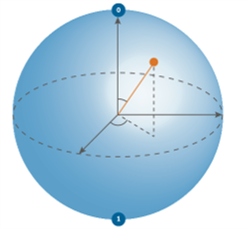
\includegraphics[width=5cm]{bloch-kugel.png}
    
\end{center}
\vfill

\footnotesize{Quelle: \url{https://www.sciencenews.org/article/quarter-century-ago-qubit-was-born}}
\end{frame}

\subsection{Superposition}
\begin{frame}
\frametitle{Superposition}
Superposition ist ein Quantenmechanisches Phänomen, welches Teilchen ermöglicht, sich in mehreren Zuständen gleichzeitig zu befinden. Dies ermöglicht Quantencomputern mehrere Rechnungen gleichzeitig durchzuführen (Quantenparallelismus), dabei nehmen Qubits erst zum Zeitpunkt der Messung einen binären Zustand ein. 
\end{frame}

\begin{frame}
\frametitle{Schrödingers Katze}
\begin{center}
    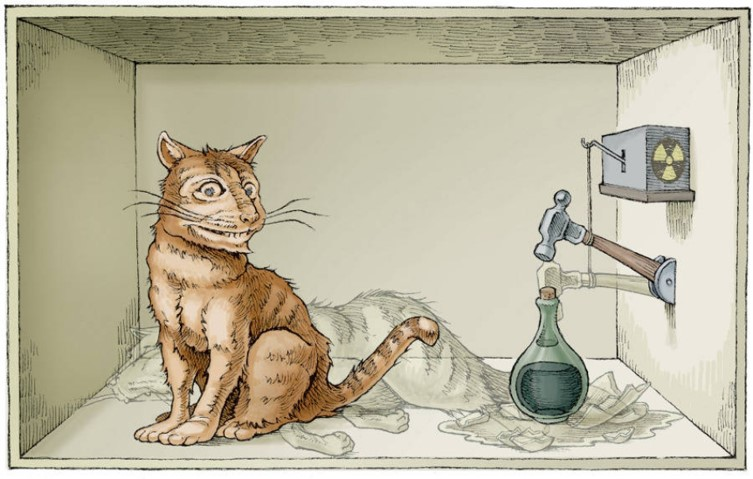
\includegraphics[width=8cm]{schroedingers.jpg}
    
\end{center}
\vfill

\footnotesize{Quelle: \url{https://www.faz.net/aktuell/wissen/physik-mehr/die-seltsame-welt-der-atome-schroedingers-katze-erhellt-das-quantenreich-12529251.html}}
\end{frame}


\subsection{Verschränkung}
\begin{frame}
\frametitle{Verschränkung}
\begin{center}
    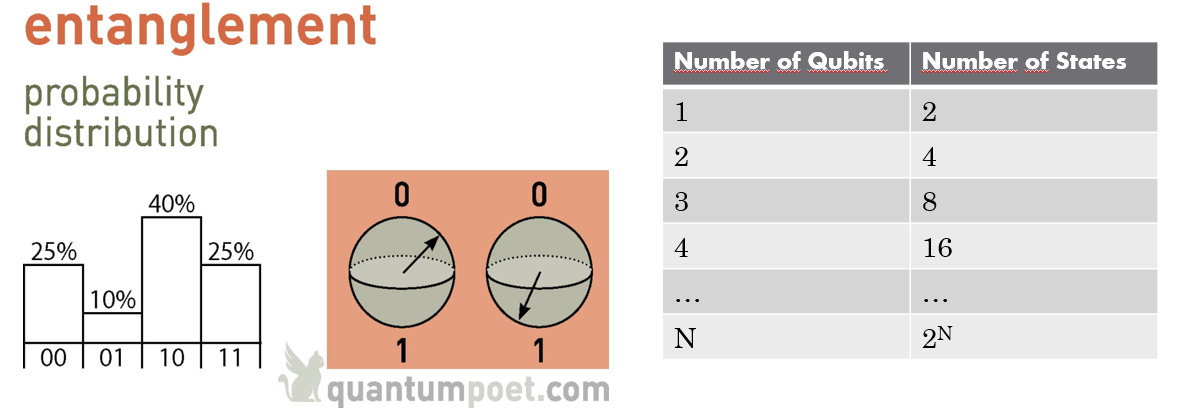
\includegraphics[width=10cm]{Verschraenkung.png}
    
\end{center}
\vfill

\footnotesize{Quelle: \url{https://quantumpoet.com/quantum-computing-introduction/}}
\end{frame}

\subsection{Interferenz}
\begin{frame}
\frametitle{Interferenz}

Qubits werden durch Quantenwellenfunktionen repräsentiert, diese beschreiben die Überlagerung verschiedener Zustände. Es können konstruktive und destruktive Interferenzmuster erzeugt werden, um das gewünschte Ergebnis zu erzielen. 

\end{frame}

\section{Kryptographie}

\subsection{Symmetrische Kryptographie}
\begin{frame}
\frametitle{Symmetrische Kryptographie}

\begin{center}
    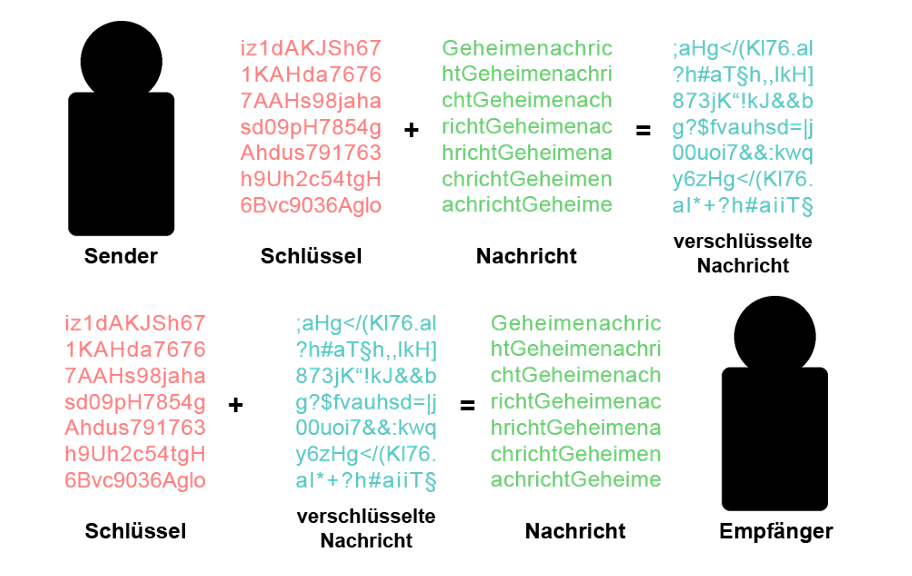
\includegraphics[width=10cm]{Symmetrische Kryptographie.png}
    
\end{center}

\end{frame}

\subsection{Asymmetrische Kryptographie}
\begin{frame}
\frametitle{Asymmetrische Kryptographie}
z.B. RSA (Rivest, Shamir, Adleman):
\begin{center}
    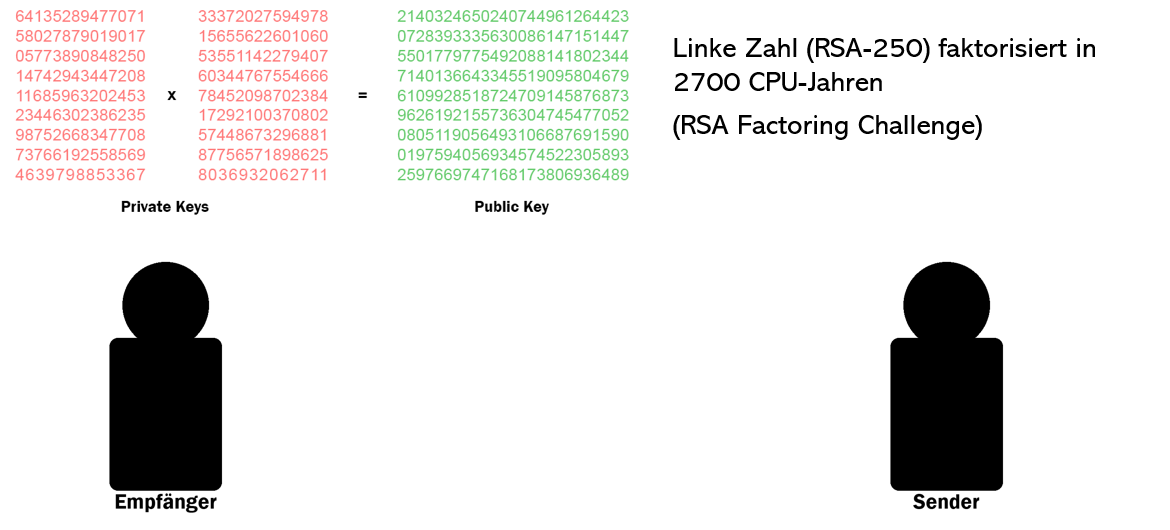
\includegraphics[width=10cm]{Asymmetrische Kryptographie.png}
    
\end{center}

\end{frame}

\subsection{Kryptographie - Vergleich}
\begin{frame}
\frametitle{Kryptographie - Vergleich}

\begin{columns}[T] % Die Option [T] sorgt dafür, dass der Inhalt beider Spalten oben beginnt

\begin{column}{.48\textwidth} % Beginn der linken Spalte
% Hier steht dein Text oder Code für die linke Spalte
\textbf{Symmetrische Kryptographie}
\begin{enumerate}
    \item[1] Gleicher, geheimer Schlüssel für Ver- und Entschlüsselung.
    \newline
    \item[2]  Standards:
    \begin{itemize}
        \item Advanced Encryption Standard (AES)
        \item Data Encryption Standard (3DES)
    \end{itemize}
    \item[]
    \item[3] Geringe Bedrohung durch Quantencomputing.
\end{enumerate}
\end{column}% Ende der linken Spalte

\begin{column}{.04\textwidth} % schmaler Zwischenraum für den vertikalen Strich
\centering
\rule{1pt}{0.7\textheight} % Vertikale Linie; passe die Höhe nach Bedarf an
\end{column}

\begin{column}{.48\textwidth} % Beginn der rechten Spalte
% Hier steht dein Text oder Code für die rechte Spalte
\textbf{Asymmetrische Kryptographie}
\begin{enumerate}
    \item[1] Unterschiedliche Schlüssel für Ver- und Entschlüsselung.
    \newline
    \item[2]  Nutzt schwierige Mathematische Probleme zur Berechnung von Schlüsseln:
    \begin{itemize}
        \item Faktorisierung (RSA)
        \item Diskreter Logarithmus
        \item ...
    \end{itemize}
    \item[3] Bedroht durch Quantencomputing.
\end{enumerate}
\end{column}% Ende der rechten Spalte

\end{columns}

\end{frame}

\subsection{Sicherheit von Verschlüsselungsmethoden}
\begin{frame}
\frametitle{Sicherheit von Verschlüsselungsmethoden}
\begin{center}
    Tabelle: Vergleich der Effektivität verschiedener
    Verschlüsselungs-Standards nach Quantencomputing
    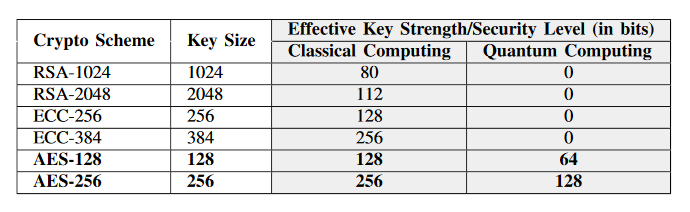
\includegraphics[width=10cm]{Tabelle.png}
    \newline
    \footnotesize{"The impact of quantum computing on present cryptography", S.4}
    
\end{center}

\end{frame}

\subsection{Shor's Algorithmus (vereinfacht)}
\begin{frame}
\frametitle{Shor's Algorithmus (vereinfacht)}

\begin{itemize}
    \item N... Nummer die faktorisiert werden soll 
    \item Wähle $x$ sodass $0 < x < N$
    \item Rechne $x$ hoch $0, 1, ..., N$
    \item Dividiere jedes Ergebnis ($x^0, x^1 x^2, ...)$ durch N und speichere den Rest
    \newline
    \item In den Resten ergibt sich eine sich wiederholende Sequenz
    \item Extrahiere (Quanten Fourer Transformation) die Periodendauer p
    \newline
    \item Möglicher Faktor $F = x^{p/2} - 1$
\end{itemize}

\end{frame}

\subsection{Folgen für Kryptographie}
\begin{frame}
\frametitle{Folgen für Kryptographie}

\begin{itemize}
    \item Meistgenutzte Verschlüsselungsverfahren werden unsicher.
    \item Quantenresistente Algorithmen nötig.
    \item Harvest now, decrypt later.
    \item Daten schon jetzt nicht mehr "sicher".
\end{itemize}
\end{frame}

\subsection{Kryptographie nach dem Quantencomputer}
\begin{frame}
\frametitle{Kryptographie nach dem Quantencomputer}

\begin{itemize}
    \item Nutzung von Quantenmechanik in der Kryptographie:
    \begin{itemize}
        \item Prepare-and-measure (Heisenbergsche Unschärferelation)
        \item Verschränkungsbasierte Protokolle (Verschränkung)
    \end{itemize}
    \item Andere mathematische Ansätze:
    \begin{itemize}
        \item Matrixmultiplikation
        \item Multivariate Polynome
        \item Hashing
        \item ...
    \end{itemize}
    \item Symmetrische Kryptographie mit größeren Schlüsseln
    \begin{itemize}
        \item z.B. Advanced Encryption Standard (AES)
    \end{itemize}
\end{itemize}

\end{frame}

\begin{frame}{Quellenverzeichnis}
\begin{itemize}
    \item \url{https://www.sciencenews.org/article/quarter-century-ago-qubit-was-born}  (Zugriff 01.04.2024)
    \item \url{https://www.faz.net/aktuell/wissen/physik-mehr/die-seltsame-welt-der-atome-schroedingers-katze-erhellt-das-quantenreich-12529251.html} (Zugriff 01.04.2024)
    \item \url{https://quantumpoet.com/quantum-computing-introduction/} Zugriff(01.04.2024)
    \item Shor, Peter W. "Quantum computing." Documenta Mathematica 1.1000 (1998): 1.
    \item Mavroeidis, Vasileios, et al. "The impact of quantum computing on present cryptography." arXiv preprint arXiv:1804.00200 (2018).
    \item \url{https://www.schneier.com/blog/archives/2020/04/rsa-250_factore.html} (Zugriff: 01.04.2024)


\end{itemize}
    
\end{frame}

\end{document}
